\section{Decoding: Greedy and Beam Search}

\begin{frame}{The Decoding Problem}
  \begin{itemize}
    \item At each step the decoder outputs a probability distribution over the vocabulary. Decoding is the search for the output sequence with the highest overall probability:
    \[
      \hat{y} = \arg\max_{y} \prod_{t=1}^{T} P(y_t \mid y_{<t}, x)
    \]
    \item Searching over all possible sequences is intractable: $|V|^T$ candidates for vocabulary size $|V|$ and length $T$.
    \item \textbf{Greedy decoding:} take the single most probable token at every step.
    \item Greedy is cheap but short-sighted: a locally best word can commit the decoder to a worse overall sentence, and there is no way back.
  \end{itemize}
\end{frame}

\begin{frame}{Beam Search}
  \begin{itemize}
    \item Keep the $k$ best partial hypotheses (the \textbf{beam}) at each step instead of just one.
    \item At every step, extend each hypothesis with every vocabulary token, score all candidates by cumulative log-probability, and keep the top $k$.
    \item $k=1$ recovers greedy decoding; machine translation typically uses beams of 4 to 10.
  \end{itemize}

  \vspace{0.4em}
  \centering
  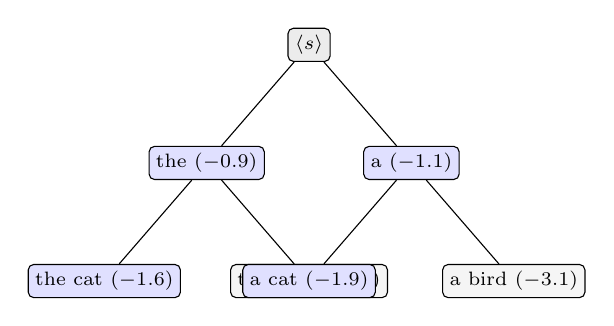
\begin{tikzpicture}[level distance=1.5cm, sibling distance=2.6cm, every node/.style={font=\scriptsize, draw, rounded corners=2pt, inner sep=2.5pt}]
    \node[fill=gray!15] {$\langle s \rangle$}
      child { node[fill=blue!12] {the ($-0.9$)}
        child { node[fill=blue!12] {the cat ($-1.6$)} }
        child { node[fill=gray!8] {the dog ($-2.8$)} }
      }
      child { node[fill=blue!12] {a ($-1.1$)}
        child { node[fill=blue!12] {a cat ($-1.9$)} }
        child { node[fill=gray!8] {a bird ($-3.1$)} }
      };
  \end{tikzpicture}

  {\scriptsize Beam of $k=2$: at each step all extensions are scored and only the two best partial sequences (blue) survive.}
\end{frame}

\begin{frame}{Beam Width Trade-offs and Length Normalization}
  \begin{itemize}
    \item \textbf{Wider beams} cost more compute and give diminishing returns; very wide beams can even hurt quality by surfacing short, generic outputs.
    \item \textbf{Length bias:} summing log-probabilities makes every added token lower the score, so beam search favors short outputs.
    \item \textbf{Length normalization} divides the score by a length penalty so hypotheses of different lengths compete fairly. Wu et al.\ (2016) use $lp(Y) = \big((5 + |Y|)/6\big)^{\alpha}$, with $\alpha$ tuned on held-out data ($\alpha = 0.2$ in that work).
    \item Beam search suits tasks with a well-defined target (translation, summarization). For open-ended generation it tends to produce repetitive, generic text, which is why sampling-based decoding is used there instead.
  \end{itemize}
\end{frame}
